\section{Struttua generale}
\label{sec:chapter_5_a_section_1}

X-Learning è una piattaforma che consente agli utenti di poter seguire/erogare corsi.
Ogni corso è caratterizzato da un categoria di interesse, descrizione, costo, materiale didattico e da un insieme di lezioni .
In generale l’utente potrà seguire le varie video lezioni contenute nel corso che rappresentato la principale fonte d’apprendimento e su cui si incentra la piattaforma.
Il processo che porta alla creazione del corso si articola in due fasi principali:
\begin{itemize}
\item Nella prima fase vengono inserite informazioni quali titolo, descrizione, linguaggio, costo e categoria obiettivi requisiti

\begin{figure}[htb]
 \centering
 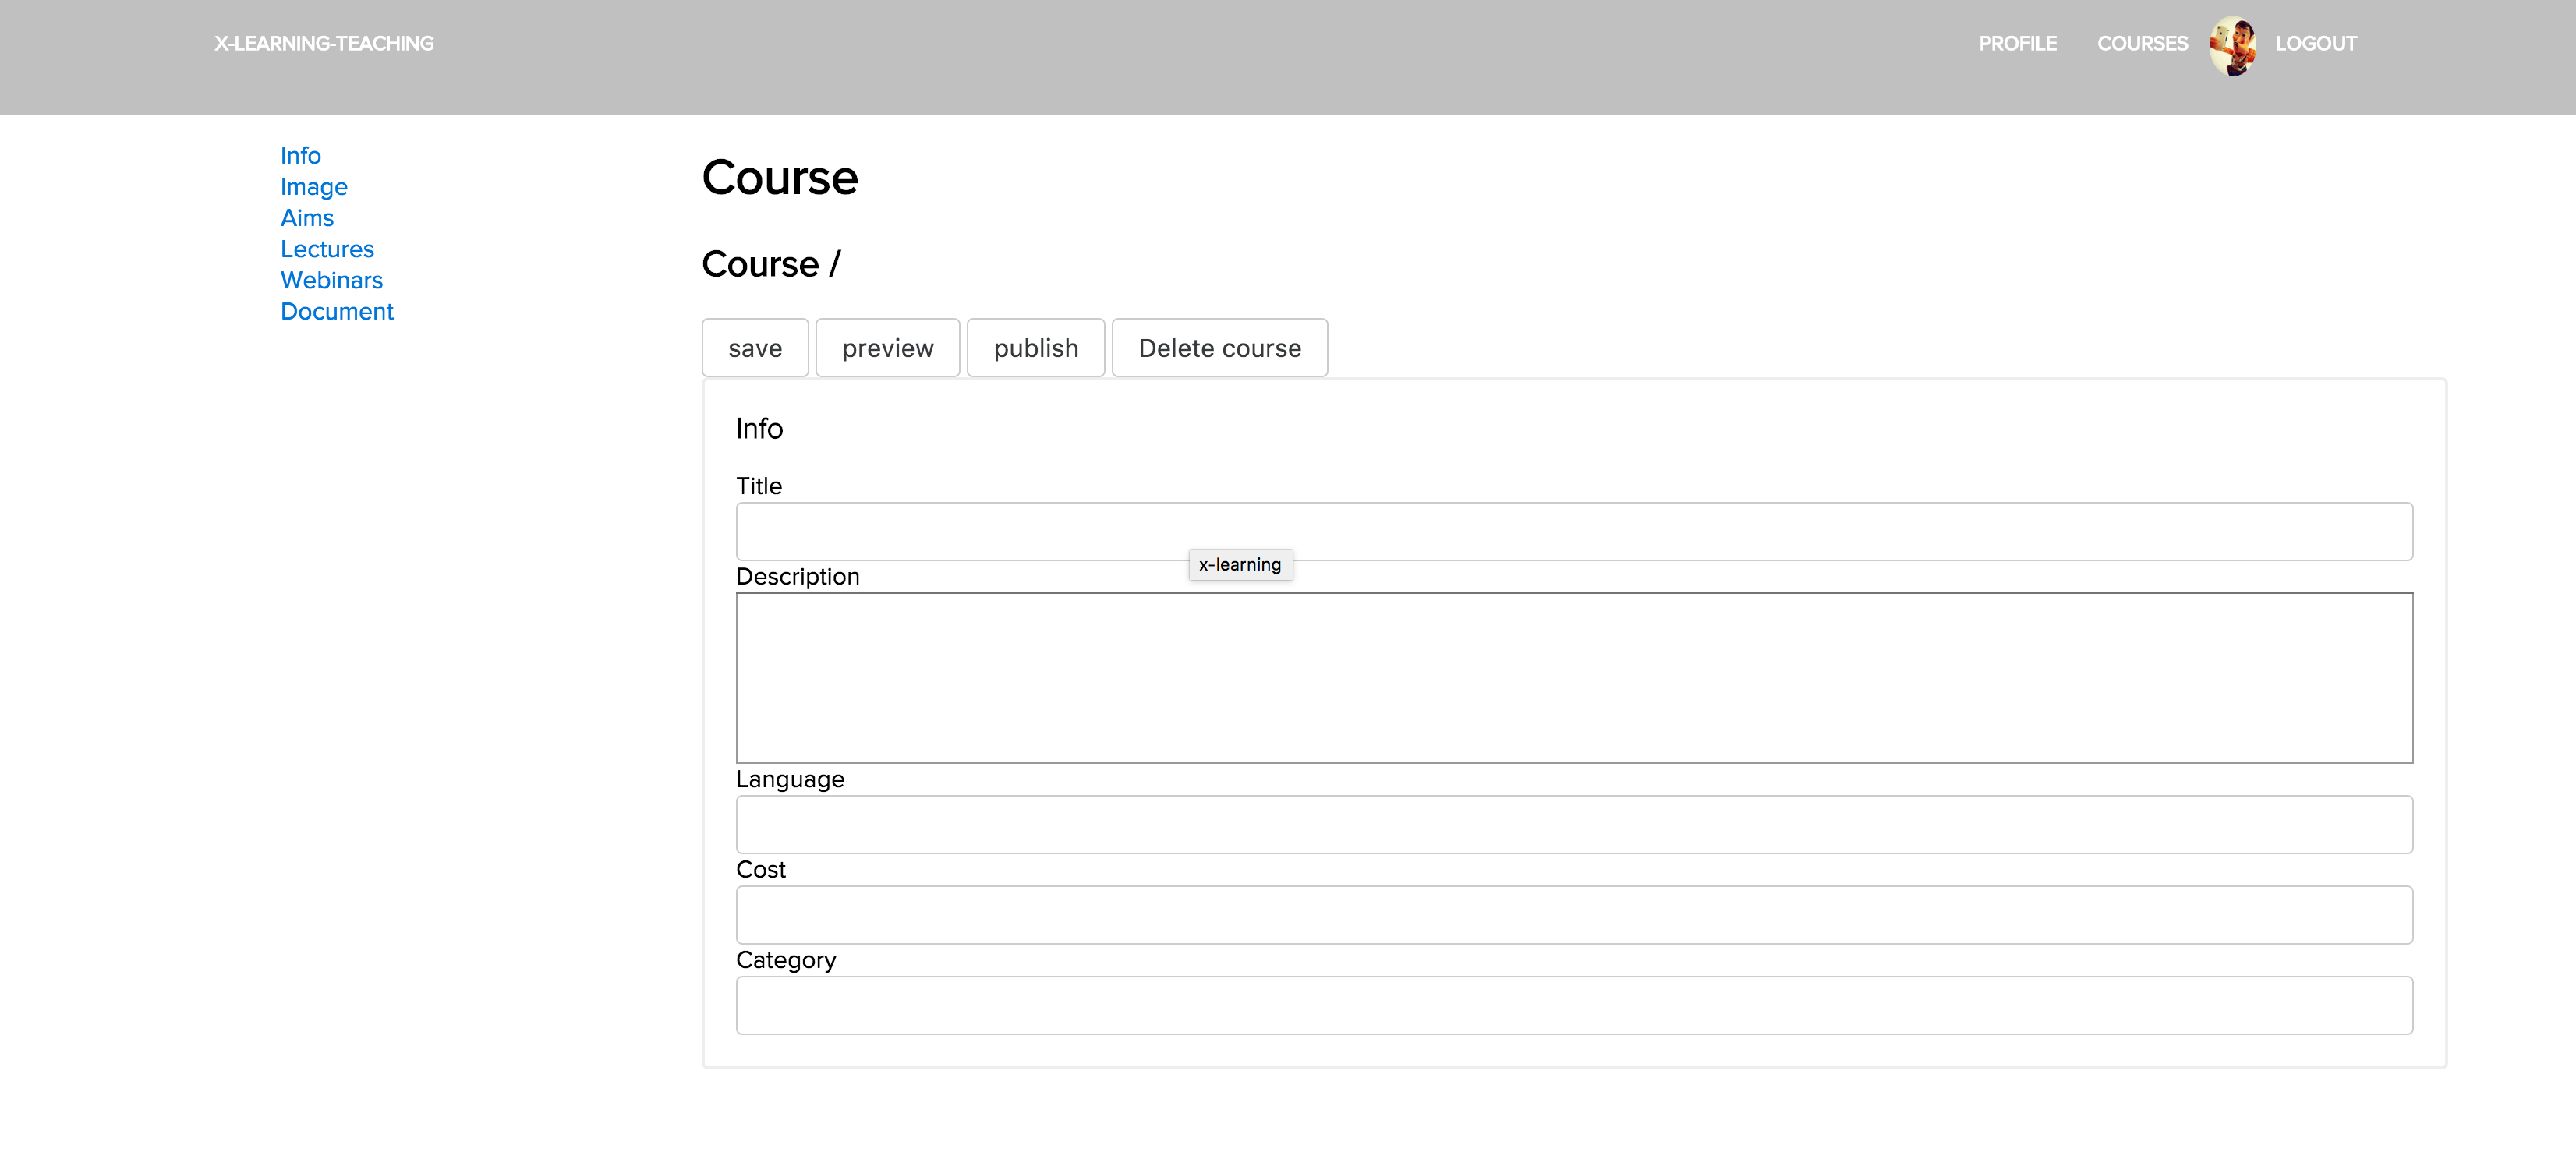
\includegraphics[width=1.0\linewidth]{images/chapter6/insert_course_page.png}\hfill
 \caption[Web Components]{Web Components}
 \label{fig:fourV}
\end{figure}

\item La seconda fase consiste nel caricare i contenuti come dati “Documents”  e creare lezioni.

\end{itemize}

Ogni lezione si contraddistinguono per titolo, descrizione ma sopratutto dal contenuto multimediale offerto.
Nei prossimi sotto capitoli verra descritto nel dettaglio il processo che porta alla creazione delle video lezioni e in particolare modo sara chiarito e dettagliato l’intero il flusso che inizia con la selezione di un determinato video da parte dell’utente. 
